\documentclass[11pt]{article}

\usepackage[spanish]{babel}
\usepackage[utf8]{inputenc}
\usepackage{amsmath, amsfonts}
\usepackage[hmargin=1.5cm, vmargin=1.5cm]{geometry}
\usepackage{graphicx}
\usepackage{titling}

\usepackage{../intro-EDP/current-definitions}

%-------------------------------------------------------------
\setlength{\droptitle}{-5em}   % Espacio antes del título
\renewcommand{\maketitlehookd}{\vspace*{-5em}} % Ejecutado después del título

\newcommand{\cabecera}{\begin{center}\it
\large
Máster en Ingeniería Naval y Oceánica, curso 2019/2020
\\[0.66em]
{\Large\bf Dinámica del Buque: CFD}
\\[0.66em]
{\bf Actividades de Evaluación}
\end{center}}
\title{\cabecera}
\author{}
\date{}
%-------------------------------------------------------------

\newcounter{actividad}
\newcommand{\actividad}[1]{
\stepcounter{actividad}
\paragraph*{Ejercicio \theactividad. #1}
}

\newcommand{\Vector}[1]{\ensuremath{\vec{\mathbf{#1}}}}
\renewcommand{\uu}{\Vector{u}}
\renewcommand{\nn}{\Vector{n}}
\newcommand{\rot}{\grad\times}
% \renewcommand{\dx}[1]{\frac{\partial #1}{\partial x}}
% \renewcommand{\dy}[1]{\frac{\partial #1}{\partial y}}

%-------------------------------------------------------------

\begin{document}

\maketitle

\begin{quotation}\small
Los siguientes ejercicios se proponen como parte de la evaluación de
la teoría de Dinámica de Fluidos Computacional (CFD).  El objetivo
último es ayudar a entender y afianzar los conceptos expuestos en
clase. Estos ejercicios se enfocan a tal efecto y por ello se ha
optado por prolongar el plazo para entregar estas actividades hasta
el día anterior la fecha del examen.  Deberán subirse a través de
la tarea que está dispuesta a tal efecto en la sección ``CFD'' del
campus virtual.
\end{quotation}

\begin{figure}
\centering
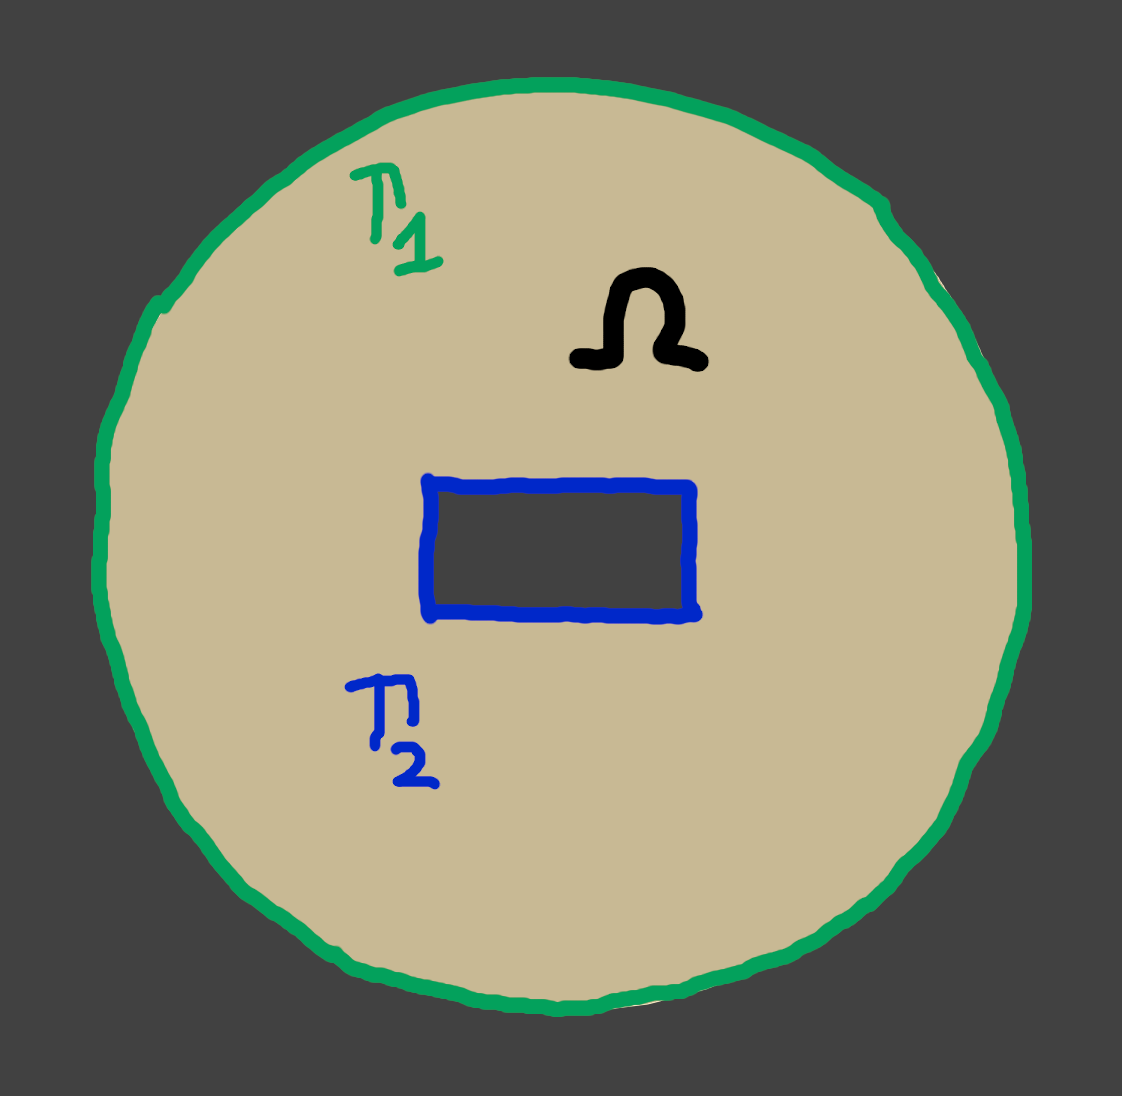
\includegraphics[width=0.25\linewidth]{dominio-circ-rect}
\caption{Dominio $\Omega$ definido por una frontera circular,
    $\Gamma_1$, que contiene a otra frontera rectangular, $\Gamma_2$.}
\label{dominio1}
\end{figure}

\actividad{} Sea el dominio $\Omega\subset\Rset^2$
(figura~\ref{dominio1}) definido por círculo con frontera
$\Gamma_1$ que contiene a un rectángulo de frontera
$\Gamma_2$. Consideramos un flujo con velocidad dada por
$$
\uu=\begin{pmatrix}
\frac{\partial\Psi}{\partial x}
\\[0.5em]
\frac{\partial\Psi}{\partial y}
\end{pmatrix},
$$
siendo $\Psi:\mathbb R^2 \to \mathbb R$ la solución del siguiente problema:
\begin{equation}
%\left\{
\begin{cases}
-\Delta\psi &=0 \quad\text{en } \Omega,
\\
\psi(x,y)&=g(x,y) \quad\forall (x,y)\in\Gamma_1,
\\
\psi(x,y)&=0 \quad\forall (x,y)\in\Gamma_2,
\end{cases}
\label{eq:psi.dirichlet}
\end{equation}
donde  $g:\Gamma_2\to\Rset$ es una función dada.

\begin{enumerate}

\item ¿De qué tipo son las condiciones de contorno enunciadas en el
caso anterior? ¿Cómo se denominan en el caso en que $g=0$? ¿Qué otro
tipo de condiciones de contorno conoces?
\item Comprobar que se verifican las siguientes propiedades: el flujo anterior es
incompresible ($\div\uu=0$) e irrotacional
($\rot\uu=0$)\footnote{Para el este flujo 2D, $\uu=(u_1,u_2)$, se
define el rotacional de $u$ como
$\rot\uu=\frac{\partial u_2}{\partial x} - \frac{\partial
    u_2}{\partial y}$.}.


\item Escribir la formulación variacional del
problema~\eqref{eq:psi.dirichlet}, para el dato de contorno
$g(x,y)=y^2$.
\begin{quotation}
\begin{footnotesize}
\begin{emph}
\textbf{Observación}: Para la formulación variacional, se recuerda la definición de los siguientes
espacios de funciones, que fueron introducidos en las clases
teóricas:
\begin{align*}
L^2(\Omega)&=\{ v:\Omega\to\Rset\ \text{tales que}\ \int_\Omega v^2 < +\infty\}
                \ \text{(funciones de cuadrado integrable en $\Omega$)},
\\
H^1(\Omega)&=\{ v:\Omega\to\Rset\ \text{tales que}\ v, \dx{v}, \dy v \in L^2(\Omega) \}
                \ \text{(funciones derivables en un sentido débil)},
\\
H^1_0(\Omega)&=\{ v:\in H^1(\Omega) \ \text{tales que}\ v=0 \text { sobre } \partial\Omega=\Gamma_1\cup\Gamma_2\}
                \ \text{(funciones de $H^1(\Omega)$ que se anulan en la frontera)}.
\end{align*}
\end{emph}
\end{footnotesize}
\end{quotation}
\vspace{-2em}
% \item Consideramos la aproximación del
%   problema~\eqref{eq:psi.dirichlet} mediante elementos finitos
%   ${\cal P}_1$. (a) Describir brevemente cómo se definen los espacios
%   polinómicos a trozos para aproximar a solución de este problema.
%   (b) La aproximación mediante elementos finitos, se obtiene como
%   solución de formulación variacional que ha sido introducida en el
%   apartado anterior? Justifica brevemente tu respuesta.


\item Escribir la formulación variacional del siguiente problema (en
  el que introducimos una condición de contorno de tipo
  deslizamiento\footnote{ Aquí $\nn(x,y)$ es el vector normal
    (exterior unitario) en cada punto $(x,y)$ de $\Gamma_2$. Por
    tanto, la condición de contorno anterior expresa que el flujo (el
    gradiente) es perpendicular al vector normal y, por tanto,
    paralelo a la frontera} en $\Gamma_2$), siendo $g$ la función dada en el
  apartado anterior:
\begin{equation*}
%\left\{
\begin{cases}
-\Delta\psi &=0 \quad\text{en } \Omega,
\\
\psi(x,y)&=g(x,y) \quad\forall (x,y)\in\Gamma_1,
\\
\grad\psi(x,y)\cdot\nn(x,y)&=0 \quad\forall (x,y)\in\Gamma_2,
\end{cases}
\end{equation*}
\end{enumerate}


\actividad{} Consideremos un flujo de Stokes en el dominio $\Omega$
definido en el ejercicio anterior (figura~\ref{dominio1}). En
concreto, planteamos: hallar un campo de velocidades $\uu=(u,v)$ y una
función presión $p$ en $\Omega\subset\Rset^2$ tales que:
\begin{align*}
- \nu\Delta u + \dx p &= f_1,
\\
- \nu\Delta v + \dy p &= f_2,
\\
\div{\uu} &  = 0,
\end{align*}
junto con condiciones de contorno en la frontera
$\partial\Omega=\Gamma_1\cup\Gamma_2$ que se detallarán a continuación. El resto de los datos son:
$\nu>0$ es la viscosidad cinemática, mientras que $f_1$ y $f_2$
denotan las dos componentes de una fuerza externa dada que
actúa sobre el flujo en $\Omega$.
%
Escribir la formulación variacional del problema anterior para
las siguientes condiciones de contorno en la frontera de $\Omega$:
\begin{enumerate}
\item $u=0, v=0$ sobre $\partial\Omega=\Gamma_1\cup\Gamma_2$ (condiciones Dirichlet homogéneas)
\item $u=y^2, v=0$ sobre $\Gamma_1$,  $u=0, v=0$ sobre $\Gamma_2$ (condiciones Dirichlet no homogéneas)
\item $u=y^2, v=0$ sobre $\Gamma_1$, $\grad\uu\cdot\nn=0$ sobre $\Gamma_2$ (condiciones mixtas Dirichlet/Neumann)
\end{enumerate}

\actividad{} Consideramos el dominio anterior
$\Omega\subset \Rset^2$ (figura~\ref{dominio1}) y un intervalo temporal $[0,T]$, siendo $T>0$
el tiempo final de observación. Definimos $\nu$ (viscosidad) y $(f_1,f_2)$ como
en el ejercicio anterior.  Planteamos: hallar $\uu=(u,v)$, donde
$u=u(x,y,t)$ y $v=v(x,y,t)$, junto a $p=p(x,y,t)$,  en $\Omega$
tales que:
\begin{align*}
\dt u - \nu\Delta u + \dx p &= f_1,
\\
\dt v - \nu\Delta v + \dy p &= f_2,
\\
\div{\uu} & = 0.
\end{align*}
junto a las condiciones de contorno homogéneas $u=v=0$ en
$\partial\Omega$.  Supongamos que el fluido parte del reposo, es decir
que tenemos las siguientes condiciones iniciales:
$$
u(x,y,0) = 0, \quad v(x,y,0)=0.
$$
\begin{enumerate}
\item Indicar en qué consiste la discretización en tiempo mediante el
esquema de Euler implícito para el problema anterior
\item Escribir la formulación variacional para dicha discretización
en tiempo.
\item Al aproximar las incógnitas de tipo velocidad y presión mediante
  elementos finitos, ¿qué tipo de espacios de funciones polinómicas a
  trozos debes elegir?
\item ¿Qué dificultades encontrarías al extender lo anterior para las
  ecuaciones de Navier-Stokes? ¿Conoces alguna forma de solucionar
  estas dificultades?

\end{enumerate}
\end{document}
